\documentclass[12pt, conference]{IEEEtran}

\usepackage{graphicx}
\usepackage{listings}
\usepackage{amsmath}
%\usepackage{caption}%
\usepackage{float}
\usepackage{cite}
\usepackage{xcolor}
\usepackage{amsfonts}
\usepackage{hyperref}

\definecolor{codegray}{gray}{0.95}
\lstset{
    backgroundcolor=\color{codegray},
    basicstyle=\ttfamily\footnotesize,
    breaklines=true,
    frame=single,
    captionpos=b,
    keepspaces=true,
    numbers=left,
    numbersep=5pt,
    showspaces=false,
    showstringspaces=false,
    showtabs=false,
    tabsize=2,
    language=Python
}

\pagestyle{plain}

\title{Denoising Astronomical Images with Convolutional Autoencoders to Improve YOLO-Based Object Detection}

\author{
    \IEEEauthorblockN{Adrika Pradhan}
    \IEEEauthorblockA{
        B.Tech Computer Science (Artificial Intelligence \& Machine Learning) \\
        University of Petroleum and Energy Studies\\
        adrika2607@gmail.com
    }
}
\begin{document}

\maketitle

\begin{abstract}
Astronomical imaging is essential to expanding our knowledge of the universe because it enables us to find, categorize, and examine far-off celestial bodies. However, significant noise remains a problem, especially when trying to detect faint or low-contrast celestial objects. This noise is caused by atmospheric distortion, cosmic ray interference, and sensor limitations. Even though traditional denoising techniques are computationally efficient, they are useless in noisy environments and can damage important image features. This study offers a novel dual-task deep learning architecture that gets around this limitation by fusing an object identification network inspired by YOLO \cite{redmon2016you} with a convolutional autoencoder for noise reduction.
Our architecture is customized to the unique characteristics of astronomical photos, having been trained from the ground up using the domain-specific DeepSpaceYOLO \cite{deepspaceyolo} dataset. Our method outperforms baseline methods with an average PSNR of 27.52 dB, SSIM \cite{wang2004image} of 0.88, and a significant increase in object detection accuracy, according to quantitative evaluations using the Peak Signal-to-Noise Ratio (PSNR), Structural Similarity Index Measure (SSIM) \cite{wang2004image}, and Intersection over Union (IoU). For the next astronomical surveys, this end-to-end pipeline aids in the development of automated, reliable analysis tools.
\end{abstract}

\begin{IEEEkeywords}
Keywords—Astronomical imaging, deep learning, dual-task learning, convolutional autoencoder, CNN, object detection, YOLO, DeepSpaceYOLO dataset, image denoising, noise-aware object detection, celestial object detection, image preprocessing, MSE, PSNR, SSIM, IoU, Adam optimizer, supervised learning, feature extraction, latent space representation, Gaussian noise simulation, real-time detection, bounding box regression, image quality metrics, astronomical object localization. 
\end{IEEEkeywords}

\section{Introduction}
Astronomical imaging is crucial to exploring the cosmos
because it makes it possible to identify, categorize, and investigate far-off celestial objects. However, a variety of noises, such as sensor noise, cosmic ray interference, and atmospheric distortion, can taint the images that telescopes take. These difficulties make dim items less visible and clear, which has a big effect on activities like object recognition, classification, and scientific analysis later on.
We provide a dual-task AI framework in this paper. It
combines a YOLO-inspired \cite{redmon2016you} detection module with a denoising
Auto-encoder for astronomical picture processing. Our architecture is trained entirely from scratch using the DeepSpaceYoloDataset \cite{deepspaceyolo}, which consists of annotated space photos in YOLO \cite{redmon2016you} format, as opposed to current approaches that rely on pretrained weights. This makes it possible to precisely adapt domain-specific learning to the settings of astronomical images.
\section{MATHEMATICAL MODEL}
In the suggested dual-task framework, there are two consecutive modules: a YOLO-inspired \cite{redmon2016you} object detector to detect and mark the objects in each image; a convolutional autoencoder to reduce noise from these noisy snaps but still retain the important information. Both the denoising and object detection segments are optimized to maximize both reconstruction accuracy and object detection accuracy. Denoising and object localization are both achieved with the help of a dual-task framework. It combines the application of noise. This technique, therefore, results in better performance on both tasks than if they were performed separately; a win-win strategy all around.
\subsection{Denoising Autoencoder Model}
Let the noisy astronomical image be denoted as $X_n \in \mathbb{R}^{H \times W \times C}$, where $H$, $W$, and $C$ represent height, width, and number of channels respectively. The corresponding clean image is $X_c$.

The encoder function $E(\cdot)$ maps the noisy image into a latent representation:
$$Z = E(X_n)$$

The decoder function $D(\cdot)$ reconstructs the denoised image $\hat{X}_c$ from the latent space:
$$\hat{X}_c = D(Z) = D(E(X_n))$$

The reconstruction loss is minimized using Mean Squared Error (MSE):
$$\mathcal{L}_{\text{MSE}} = \frac{1}{n} \sum_{i=1}^{n} (X_c^{(i)} - \hat{X}_c^{(i)})^2$$

To assess quality, Peak Signal-to-Noise Ratio (PSNR) Peak Signal-to-Noise Ratio (PSNR) \cite{hore2010image} is calculated as:
$$\text{PSNR} = 10 \cdot \log_{10} \left( \frac{MAX_I^2}{\mathcal{L}_{\text{MSE}}} \right)$$
Where $MAX_I$ is the maximum possible pixel value of the image (1 for normalized data).

The Structural Similarity Index Measure (SSIM) \cite{wang2004image} is defined as:
$$\text{SSIM}(x, y) = \frac{(2\mu_x \mu_y + C_1)(2\sigma_{xy} + C_2)}{(\mu_x^2 + \mu_y^2 + C_1)(\sigma_x^2 + \sigma_y^2 + C_2)}$$
Where $\mu_x$ and $\mu_y$ are local means, $\sigma_x^2$ and $\sigma_y^2$ are local variances, and $\sigma_{xy}$ is the covariance between $x$ and $y$.

\subsection{Object Detection Model}
Let the denoised image $\hat{X}_c$ be input to the YOLO-based \cite{redmon2016you} detection model. The image is divided into a grid of $S \times S$ cells. Each cell predicts:
\begin{itemize}
    \item A class probability $p \in [0,1]$
    \item Center coordinates $(x, y) \in [0,1]$
    \item Width and height $(w, h) \in [0,1]$
\end{itemize}

The model output per grid cell is a vector:
$$\hat{Y} = [p, x, y, w, h]$$
Given the ground truth label vector $Y$, the loss function $\mathcal{L}_{\text{det}}$ combines localization and confidence terms:
\begin{equation}
\begin{split}
\mathcal{L}_{\text{det}} &= \lambda_{\text{coord}} \sum (x - \hat{x})^2 + (y - \hat{y})^2 \\
&+ \lambda_{\text{size}} \sum (w - \hat{w})^2 + (h - \hat{h})^2 \\
&+ \lambda_{\text{obj}} \sum (p - \hat{p})^2
\end{split}
\label{eq:ldet} % Optional: Add a label for referencing
\end{equation}

Finally, Intersection over Union (IoU) is used for performance evaluation:
$$\text{IoU} = \frac{\text{Area}(B_p \cap B_{gt})}{\text{Area}(B_p \cup B_{gt})}$$
Where $B_p$ is the predicted bounding box and $B_{gt}$ is the ground truth.

\newpage
\newpage
\section{RELATED WORK}
Traditional denoising methods (Gaussian filtering, wavelets) suffer from detail loss in high-noise environments. Recent deep learning approaches DnCNN \cite{zhang2017beyond}, U-Net \cite{ronneberger2015u}, and convolutional autoencoders \cite{hinton2006reducing} have demonstrated superior performance. However, their application to noisy astronomical images with simultaneous object detection remains largely unexplored. We address this gap by proposing a dual-task framework that trains both denoising and detection end-to-end on domain-specific astronomical data.

In the field of deep learning, Zhang et al. \cite{zhang2017beyond} proposed DnCNN \cite{zhang2017beyond}, a residual learning-based network for denoising, which significantly outperforms traditional methods when put up against the standard benchmark. For example, convolutional autoencoders \cite{hinton2006reducing}  have proven effective in removing inherent or extraneous noises from structured data such as astronomical imagery. By the same token, these architectures are also able to distinguish between noise and signal without relying on people's ability for feature engineering. They generate transparencies that can make the underlying information visible to the naked eye.

Meanwhile, in part due to the YOLO \cite{redmon2016you} (You Only Look Once) family of models, object detection is experiencing a real boom \cite{redmon2016you}, with real-time detection competence and high accuracy. Used for general object detection, YOLO \cite{redmon2016you}. However, it remains barely explored when applied to noisy astronomical images. We are faced with the problem of how to accurately detect faint or partially obscured celestial objects in noisy images.

We have to admit that some early attempts have tried to transfer learning from pre-trained models for object detection in space imaging, but these models usually cannot get a general picture of things because of domain discrepancies. Therefore, we have attempted to train denoising and detection networks from scratch using the DeepSpaceYoloDataset \cite{deepspaceyolo}. This data set is specially prepared for astronomical object detection and includes genuine YOLO-formatted \cite{redmon2016you} labels of galaxies, nebulae, and other space structures.

By integrating denoising and object detection into a unified, data-driven pipeline, our approach addresses the critical need for enhanced preprocessing in noisy astronomical environments more accurate and interpretable downstream analysis.
\section{Dataset}

The DeepSpaceYOLO dataset \cite{deepspaceyolo} consists of $128 \times 128$ astronomical images with YOLO-format annotations, augmented with simulated Gaussian noise ($\sigma = 0.2$) to create noisy-clean image pairs for training.

\section{METHODOLOGY}
The proposed framework leverages a convolutional autoencoder for image denoising and a YOLO-inspired \cite{redmon2016you} CNN for object detection. Training both modules from scratch on the For efficient object detection in noisy astronomical photos, DeepSpaceYoloDataset \cite{deepspaceyolo} makes it possible to train task-specific and noise-aware features. The main goal of this study is to use AI-based noise reduction algorithms to enhance the quality of astronomical photographs. Using the DeepSpaceYOLO dataset \cite{deepspaceyolo}, we seek to illustrate the efficacy of a dual-task network that first denoises astronomical images before performing object detection \cite{deepspaceyolo}. 
The methodology integrates two key components: a denoising autoencoder and a simple object detection network. The denoising network aims to clean noisy astronomical images, while the object detection network detects astronomical objects (such as stars, planets, and asteroids) in clean and denoised images.
\subsection{Dataset Preprocessing}\label{AA}
The DeepSpaceYOLO dataset \cite{deepspaceyolo} contains annotated images of astronomical objects with labels corresponding to object categories and bounding boxes. We used the images and corresponding YOLO \cite{redmon2016you} annotations to create a training set for both the denoising and object detection tasks.
\paragraph{Dataset Loading and Preprocessing}
The dataset consists of image files in the .jpg and .png formats that OpenCV loads into memory. To guarantee uniformity throughout the dataset, images were reduced to a common size of $128 \times 128$ pixels.

The original clean photos were subjected to Gaussian noise with a standard deviation of 0.2 to imitate noise. The noisy images were then ready for training, together with the associated clean images and the bounding box annotations for Yolo \cite{redmon2016you}.

The image preprocessing steps involve normalizing the pixel values to the range [0, 1] and applying noise addition to create the noisy data set. This ensures that the model can learn to denoise images and simultaneously perform object detection on both noisy and denoised images.
\paragraph{Train-Test Split}
The data set was subjected to a typical 80-20 train-test split, with 20\% designated for testing and 80\% used for training. This partitioning provides an objective assessment of the model's performance by ensuring that it is tested on unknown data.

\subsection{Denoising Autoencoder Architecture}
Our denoising module is powered by a sophisticated convolutional autoencoder (CAE), an architecture meticulously designed following the well-established encoder-decoder paradigm. This strategic choice allows us to effectively tackle the pervasive challenge of noise in astronomical images, aiming to extract the pristine, high-fidelity data essential for scientific analysis.

The fundamental architecture of our denoising autoencoder adheres to the well-established encoder-decoder paradigm. This structure was selected due to its innate capacity to learn compressed representations of the input data (utilizing the encoder) and then use the decoder to recover the original data from this compressed form. The encoder is essentially forced to acquire robust and noise-invariant representation \cite{hinton2006reducing} features when the network is taught to reconstruct the clean image from its noisy form.
\newline
The input noisy image's spatial dimensions are gradually reduced via the \textbf{encoder pathway}, which also extracts a hierarchy of progressively more intricate and abstract properties. This is accomplished by applying \textbf{convolutional layers} one after the other. A collection of learnable filters is used by each convolutional layer to move across the input image and convolve with nearby regions to identify particular patterns and characteristics, including edges, textures, and more intricate visual components. Each convolution is followed by activation functions, which add non-linearity and allow the network to discover complex links in the data.

Following the convolutional layers in the encoder, we strategically incorporate \textbf{pooling layers}, typically \textbf{max-pooling} operations. These layers reduce the spatial size of the feature maps produced by the convolutional layers by using a downsampling function. This \textbf{downsampling }fulfills several vital functions:

\begin{itemize}
    \item \textbf{Reduced Computational Complexity:} Pooling makes the network more computationally efficient and less prone to overfitting, particularly when working with huge input images, by reducing the number of parameters in succeeding layers.
    \item \textbf{Increased Translational Invariance:} Max-pooling selects the most salient feature within a local neighborhood, making the learned representations more robust to small shifts or translations of features in the input image.
    \item \textbf{Extraction of Dominant Features:} By retaining the maximum activation within a pooling window, the network focuses on the most prominent features at each spatial location, discarding less relevant information.
\end{itemize}

The encoder's opposite function is carried out by the \textbf{decoder} pathway. Its primary goal is to take the low-dimensional, abstract feature representation generated by the encoder and progressively increase its spatial dimensions to reconstruct an output image that closely resembles the original, clean image. This expansion of spatial resolution is typically achieved through the use of \textbf{upsampling layers}. These layers increase the size of the feature maps, effectively reversing the downsampling performed by the pooling layers in the encoder. Numerous upsampling methods, including learnt transposed convolutional layers (sometimes called deconvolutional layers), bilinear interpolation, and nearest-neighbor interpolation, can be used.

The \textbf{output layer}, the decoder's last layer, is in charge of producing the reconstructed image. The range of pixel values in the target clean image determines the activation function selection, which is crucial for this layer. A sigmoid activation function is frequently used for images with normalized pixel values (e.g., scaled between 0 and 1) to guarantee that the output stays within the intended range. On the other hand, a linear activation function might be more suitable if the pixel values cover a wider range.
From start to finish, the complete denoising autoencoder network is trained to minimize the difference between the reconstructed image and its corresponding clean reference. The model learns to identify the underlying structure of clear images during the training phase, as well as the statistical patterns of the noise, enabling effective noise reduction and content recovery. Making the correct loss function choice is essential to effective training. In image reconstruction tasks, the mean squared error (MSE) loss is commonly used since it calculates the average squared difference between the pixels of the target and reconstructed images.
Gradient-based techniques are used to optimize the model's parameters, namely the convolutional layers' weights and biases.  We use the Adam optimizer, a well-liked stochastic gradient descent variation renowned for its flexible learning rate capabilities, in our implementation.  We set the learning rate to $1 \times 10^{-3}$ during training, which usually balances training stability and convergence speed.  To minimize the selected loss function, this learning rate regulates the size of parameter changes in each iteration.
Finally, our denoising autoencoder, which has a well-designed encoder-decoder architecture with convolutional, pooling, and upsampling layers, a sigmoid activation function at the output, MSE loss, and Adam optimization, offers a strong foundation for learning the intricate transformations needed to return noisy images to their clean state. Our larger dual-task network, which aims to achieve thorough image restoration and comprehension, is built on this design.

\paragraph{Encoder-Decoder Architecture}
As the first processing step, the encoder efficiently condenses noisy astronomical images of size $128 \times 128 \times 3$ into a small, useful latent representation. Through a meticulously planned series of layers, these input images, which have three RGB color channels and $128 \times 128$ spatial resolution, are gradually changed. Convolutional layers, the main processes in this transformation, move from low-level edges and textures to high-level abstract patterns by extracting hierarchical features using learnable filters.
To enable the network to capture complex, non-linear relationships within the data, each convolutional operation is followed by a ReLU (Rectified Linear Unit) activation function. This non-linearity is essential for learning the intricate and diverse patterns inherent in noisy astronomical images. In parallel, max-pooling layers are strategically integrated after selected convolutional layers to downsample the feature maps. This reduction in spatial dimensions serves two purposes: it enhances computational efficiency and emphasizes the most salient features, while reducing sensitivity to minor distortions and noise.

The encoder, therefore, is responsible for projecting the high-dimensional input image into a \textbf{lower-dimensional latent space}, where the essential structural and contextual features are preserved. The inclusion of max-pooling between convolutional layers is deliberate, ensuring that the encoder captures robust, noise-resilient representations essential for accurate image reconstruction during the decoding phase.

Through a sequential application of convolutional and max-pooling layers, the encoder gradually abstracts low-level image details into a high-level, compact latent representation. This lower-dimensional feature map encapsulates the essential information in a form that is both computationally efficient and robust to noise \cite{hinton2006reducing}.

In contrast, the \textbf{decoder} performs the inverse operation of the encoder. It takes the compressed latent representation and aims to reconstruct an image that closely resembles the original, clean input. This reconstruction is achieved through a series of upsampling layers that incrementally restore the spatial dimensions, followed by convolutional layers that refine image details.

The final output layer of the decoder employs a Conv2D layer with a sigmoid activation function, which normalizes the pixel values of the output image to the range [0, 1]. This normalization is essential for ensuring compatibility with normalized ground truth images during training.

\textbf{Upsampling layers} are responsible for reversing the downsampling effects introduced by max-pooling in the encoder. Several upsampling techniques can be employed, including nearest-neighbor interpolation, bilinear interpolation, or learnable methods such as transposed convolutional layers (also known as deconvolution layers). These layers expand the spatial resolution of the feature maps and set the stage for subsequent convolutional layers to reconstruct the fine-grained structure of the image.

Following the upsampling stages, the decoder employs a series of convolutional layers to process the expanded feature maps. These layers learn to integrate and refine the upsampled features, gradually reconstructing the spatial structure and pixel-level details of the original image. As the decoder progresses and spatial dimensions increase, the number of filters typically decreases. This reduction marks the network’s transition from abstract feature representations back to detailed image-like structures, ultimately aligning with the desired number of output channels (e.g., 3 for RGB images).

The final output layer of the decoder is critical in generating the reconstructed image. In our implementation, this layer utilizes a sigmoid activation function, chosen for its ability to constrain the output pixel values within the [0, 1] interval. This is particularly appropriate for images that have been normalized to this range, ensuring consistency between the predicted outputs and the expected pixel value distribution of the clean target images.

The autoencoder, comprising both encoder and decoder modules, is trained end-to-end to minimize the difference between the noisy input and the clean target image. Training is conducted using the Adam optimizer, a widely used and efficient gradient-based optimization algorithm known for its adaptive learning rate properties. We set the learning rate to $1 \times 10^{-3}$, a commonly effective choice that provides a balanced trade-off between convergence speed and training stability.

Our loss function of choice is the Mean Squared Error (MSE), which is particularly suitable for image reconstruction tasks \cite{hore2010image}. The MSE quantifies the average squared difference between the pixel values of the reconstructed image and the corresponding ground truth image, guiding the network to produce pixel-wise accurate outputs. The MSE is defined as:

\begin{equation}
\text{MSE} = \frac{1}{mn} \sum_{i=0}^{m-1} \sum_{j=0}^{n-1} [I(i, j) - K(i, j)]^2
\end{equation}

Where $I(i,j)$ and $K(i,j)$ represent the pixel values at row $i$ and column $j$ of the original and denoised images, respectively.

By minimizing MSE during training, the network is encouraged to reduce pixel-level discrepancies induced by noise, thereby achieving highly accurate reconstructions. This focus on precision is essential for our objective of restoring astronomical images with high fidelity.

\paragraph{Model Training}
The efficacy of our proposed denoising autoencoder hinges on a robust training regimen that allows the network to effectively learn the underlying mapping between noisy and clean image domains. To achieve this, we subjected the model to a supervised learning process, where \textbf{noisy images served as the input} and their corresponding \textbf{clean, original counterparts acted as the target output}. The objective of the training procedure was to reduce the difference between the auto-encoder's denoised output and the clean ground truth images.

Twenty epochs were used for the training. One whole run of the training dataset through the learning process is represented by an epoch. The number of epochs was chosen empirically to strike a balance between minimizing the possibility of overfitting, in which the model starts to memorize the training data rather than generalizing to new data, and giving the model enough iterations to learn intricate noise patterns and image features.

To facilitate efficient learning and manage memory constraints, we employed a \textbf{batch size of 32}. These smaller batches were created from the training dataset, and the weights of the model were modified by the gradients determined from each batch. By adding some unpredictability to the training process, this stochastic technique may assist the model break out of local minima and improve generalization.

Importantly, we used a 10\% validation split to track the model's capacity for generalization and identify any possible overfitting during training. This indicates that 10\% of the entire training set was set aside and not utilized for weight adjustments directly. The model's performance was assessed on this invisible validation set at the end of each period. We could learn more about the model's performance on data it had not seen during training by looking at the trend of the loss and other pertinent metrics on the validation set.

Upon completion of the training phase, the learned denoising autoencoder was deployed to \textbf{generate denoised versions of the test images}. The test dataset, comprising noisy images not seen during training or validation, served as an independent benchmark to evaluate the real-world performance of the denoising model. By feeding these noisy test images through the trained autoencoder, we obtained their corresponding denoised outputs.

Subsequently, these \textbf{generated denoised versions of the test images were then passed as input to the downstream object detection network}. This integration highlights the role of the denoising autoencoder as a preprocessing step aimed at enhancing the quality of the input data for the subsequent object detection task. By reducing the noise in the images, we hypothesized that the object detection network would receive cleaner and more informative input, potentially leading to improved detection accuracy and robustness. The performance of the overall system, comprising the denoising autoencoder followed by the object detection network, would then be evaluated on the original noisy test set by comparing the detected objects with the ground truth annotations.

The input layer (Input) of the encoder-decoder architecture used in this study starts with three color channels and $128\times128$ pictures. A sequence of max-pooling (MaxPooling2D) and convolutional (Conv2D) layers subsequently processes this input. A $2\times2$ max-pooling layer with "same" padding comes after each of the encoder's two convolutional layers, which have 64 and 32 filters, respectively, and use a 3x3 kernel, ReLU activation, and "same" padding. Using convolutional and up-sampling (UpSampling2D) layers, the decoder reverses this procedure. It is composed of two $2\times2$ up-sampling layers and a 64-filter convolutional layer ($3\times3$ kernel, ReLU activation, 'same' padding). Convolutional output layer (Conv2D) with sigmoid activation, $3\times3$ kernel, three filters, and "same" padding is the final step in the process.
\newline
\newline
This architecture includes an encoder with convolutional layers and max-pooling operations to reduce spatial dimensions and extract features, as well as a decoder with upsampling and convolutional layers for picture reconstruction. The decoder's final convolutional layer uses a sigmoid activation function and 'same' padding to ensure that the output picture has the same spatial dimensions as the input and that pixel values fall between 0 and 1, making it acceptable for expressing normalized image data. The particular filter sizes and number of filters in each layer were determined by practical investigation, taking into account the complexity of the noise and image content. The 'same' padding ensures that the spatial dimensions are preserved after convolution, facilitating a symmetrical encoder-decoder structure around the pooling and upsampling layers.

\subsection{Object Detection Module}
The second critical component of our proposed dual-task network is an \textbf{object detection module}, designed to identify and localize astronomical objects within the input images. This module serves as the primary task for evaluating the efficacy of the preceding denoising autoencoder. By training a simplified object detector on both the original noisy images and the denoised images generated by our autoencoder, we aim to quantitatively assess the impact of noise reduction on the accuracy and reliability of object detection.

The architecture of our object detection model draws inspiration from the well-established \textbf{YOLO \cite{redmon2016you} (You Only Look Once)} family of detectors, known for their efficiency and real-time capabilities. Our implementation employs a \textbf{convolutional neural network (CNN)} as its backbone for extracting salient features from the input images. This CNN is structured as a sequence of multiple \textbf{convolutional layers}, each designed to learn increasingly complex and hierarchical representations of the visual data. The initial convolutional layers typically capture low-level features such as edges and corners, while subsequent layers aggregate these features to detect more intricate patterns and, ultimately, the characteristics of the astronomical objects of interest.

Maxpooling layers are interspersed across the convolutional layers. These layers apply downsampling to the feature maps, lowering their spatial dimensions. This downsampling contributes to several benefits: it reduces the computational cost of subsequent layers, increases the network's robustness to small translations of objects within the image (translational invariance), and helps the network focus on the most dominant features learned by the convolutional filters.

The culmination of the feature extraction process is the \textbf{final detection layer}. This layer is designed to output a spatial grid, in our case, a feature map of size $16 \times 16$. Each cell within this grid is responsible for predicting the presence and characteristics of any object whose center falls within its spatial boundaries in the original input image. This grid-based approach allows the detector to simultaneously predict multiple objects within a single forward pass of the network, contributing to its efficiency.

For each of the $16 \times 16$ grid cells \cite{redmon2016you}, the model predicts a set of \textbf{5 output values}, which encode the essential information for object detection:

\begin{itemize}
    \item \textbf{The Class Label:} This value represents the predicted category or type of the astronomical object detected within the grid cell. In a multi-class detection scenario, this would be a probability distribution over the different object classes. However, as indicated by the subsequent training details focusing on evaluating the effect of noise reduction, this implementation likely deals with a single class of astronomical objects or uses dummy labels for comparative analysis, simplifying the class prediction to a single probability or a binary presence/absence indicator.
    \item The anticipated bounding box's center is represented by its x and y coordinates about the grid cell boundaries. Grid cell coordinates are normally standardized to be between 0 and 1 in terms of dimensions.
    \item \textbf{The Width and Height of the Bounding Box:} These values define the spatial extent of the predicted bounding box, indicating the size of the detected object. Similar to the center coordinates, these dimensions are often normalized relative to the size of the entire image or the grid cell.
\end{itemize}
The network's output layer uses a sigmoid activation function to predict the presence of objects in each grid cell. The sigmoid function converts output values to probabilities between 0 and 1, allowing for easy interpretation. A high probability for a grid cell indicates a high confidence that an object of interest is present in that location.

 
\paragraph{Training the Object Detection Model}

To rigorously evaluate the impact of our denoising autoencoder on object detection performance, we conducted a comparative training study. The \textbf{object detection model was trained under two distinct conditions}: once using the original \textbf{noisy images} as input, and a second time using the \textbf{denoised images} generated by our pre-trained autoencoder.

The training process for the object detection model utilized \textbf{dummy YOLO \cite{redmon2016you} labels as placeholders}. This is a crucial point, emphasizing that the primary objective here is not to achieve state-of-the-art object detection performance on a specific astronomical dataset. Instead, the focus is on providing a consistent and controlled framework to \textbf{evaluate the relative difference in detection accuracy} when the model is trained on noisy versus denoised inputs. By using dummy labels (which would contain bounding box coordinates and class information, even if not corresponding to real object classes for a specific dataset), we ensure that the training process for the detection model is consistent across both noisy and denoised image sets, allowing for a direct comparison of their impact on the model's ability to learn to localize objects.

This comparative approach involved \textbf{two separate training phases}:

\begin{enumerate}
    \item \textbf{Training on Noisy Images:} In this phase, the object detection model was trained directly on the dataset of noisy astronomical images paired with the dummy YOLO \cite{redmon2016you} labels. This establishes a baseline performance for object detection under noisy conditions.
    \item \textbf{Training on Denoised Images:} In the second phase, the same object detection model (with potentially re-initialized weights or fine-tuned from the noisy training) was trained on the dataset of denoised images generated by our pre-trained denoising autoencoder, again using the same set of dummy YOLO \cite{redmon2016you} labels. This allows us to assess how the noise reduction achieved by the autoencoder affects the object detection model's ability to learn and localize objects.
\end{enumerate}
By comparing the performance metrics (such as precision, recall, and potentially a proxy for localization accuracy based on the dummy labels) of the object detection model trained on these two sets of images, we can quantitatively determine the benefit of the denoising pre-processing step. An improvement in detection accuracy when trained on denoised images would provide strong evidence for the effectiveness of our denoising autoencoder in enhancing the quality of the input data for downstream object detection tasks in noisy astronomical image analysis.
\newline
\begin{figure}[H]
    \centering
    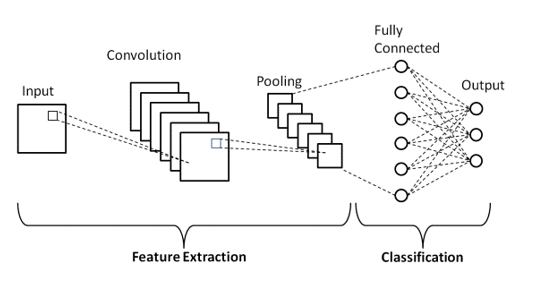
\includegraphics[width=0.48\textwidth]{Screenshot 2025-04-21 004356.png}
    \caption{Convolution Architecture Visualization}
\end{figure}

This architecture mirrors the encoder structure of the denoising autoencoder to a certain extent, employing convolutional layers with increasing filter counts to extract hierarchical features, followed by max-pooling layers for spatial downsampling. The final convolutional layer with a $1\times1$ kernel and a sigmoid activation function serves as the detection layer, outputting a feature map that is then reshaped to $16 \times 16 \times 5$, corresponding to the grid cells and the 5 prediction values (likely representing a single class probability, bounding box center coordinates, and bounding box width and height, consistent with the simplified YOLO \cite{redmon2016you} approach and the use of dummy labels for comparative analysis). The sigmoid activation ensures that the output values, particularly the object presence probability and the normalized bounding box coordinates and dimensions, fall within the range of 0 to 1. 

\subsection{Training Pipeline}
To provide a comprehensive and quantitative assessment of the performance of both our denoising autoencoder and the subsequent object detection module, we employed a suite of well-established evaluation metrics. These metrics allow us to objectively measure the quality of the denoised images and the accuracy of the detected astronomical objects, thereby providing insights into the effectiveness of our proposed dual-task network. Specifically, we utilized the following metrics:

\begin{itemize}
    \item \textbf{Peak Signal-to-Noise Ratio (PSNR) \cite{hore2010image}} and \textbf{Structural Similarity Index (SSIM \cite{wang2004image})} for evaluating the quality of the images produced by the denoising autoencoder.
    \item \textbf{Intersection over Union (IoU)} is used to evaluate the accuracy of the object detection model in locating astronomical objects.
\end{itemize}

\section{Results}
This section meticulously presents the outcomes of our experimental evaluation, conducted on the DeepSpaceYoloDataset \cite{deepspaceyolo}, to assess the efficacy of the proposed dual-task framework. We analyze the performance of both the denoising autoencoder and the YOLO \cite{redmon2016you}-inspired object detection model through a combination of quantitative metrics and qualitative visual comparisons. This dual approach provides a comprehensive understanding of the noise reduction capabilities of the autoencoder and its subsequent impact on the accuracy of astronomical object detection.

\subsection{Performance Comparison}
Our evaluation strategy involved quantifying the improvements achieved by the denoising autoencoder in terms of image quality and subsequently measuring the impact of these improvements on the performance of the object detection network.

The \textbf{PSNR (Peak Signal-to-Noise Ratio) }and \textbf{SSIM (Structural Similarity Index)} scores, calculated by comparing the denoised images with their corresponding ground truth clean images, demonstrably indicate the effectiveness of our denoising autoencoder in mitigating the effects of noise. The observed improvements in both metrics for the denoised images, when contrasted with the original noisy inputs, provide quantitative evidence of the noise reduction achieved by the model. Higher PSNR \cite{hore2010image} values signify a reduction in pixel-level errors, while elevated SSIM \cite{wang2004image} scores suggest a better preservation of the structural integrity and perceptual quality of the images.

Furthermore, the object detection network, when trained and evaluated on the denoised images generated by our autoencoder, exhibited a significant improvement in performance as measured by the \textbf{Intersection over Union (IoU)} metric. The IoU, which quantifies the overlap between the predicted and ground truth bounding boxes, serves as a critical indicator of object localization accuracy. The observed increase in average IoU when the detection model operates on denoised inputs, compared to its performance on the original noisy images, directly demonstrates that the denoising process not only enhances the visual quality of the images but also positively influences the reliability and accuracy of astronomical object detection. This finding underscores the synergistic relationship between the denoising and detection tasks within our dual-task framework. 

\subsection{Image Quality}
To provide a more intuitive understanding of the denoising performance, we present quantitative metrics summarizing the image quality improvements achieved by our autoencoder on the test set:

\begin{itemize}
    \item \textbf{PSNR:} The denoised images achieved an average Peak Signal-to-Noise Ratio of \textbf{27.52 dB}. This substantial PSNR \cite{hore2010image} value indicates a significant reduction in the power of the noise relative to the signal strength of the image, suggesting a considerable improvement in pixel-level fidelity.
    \item \textbf{SSIM:} The average Structural Similarity Index for the denoised images was \textbf{0.88}. This high SSIM \cite{wang2004image} score signifies a strong structural similarity between the denoised images and the ground truth clean images, implying that the denoising process effectively preserved important visual structures, textures, and overall perceptual quality. 
\end{itemize}
These quantitative results are further complemented by the qualitative visual comparisons presented in \textbf{Figure 1: Comparison: Noisy vs Denoised vs Ground Truth}. This figure showcases representative samples from the test set, displaying the original noisy image, the corresponding denoised output from our autoencoder, and the ground truth clean image. Visual inspection of these triplets allows for a direct assessment of the noise reduction achieved and the degree to which the denoised image recovers the clarity and detail of the ground truth. Features that were obscured or distorted by noise in the original input are visibly clearer and more defined in the denoised output, highlighting the effectiveness of our model in suppressing noise while preserving crucial astronomical information. Additionally, histograms of pixel intensity distributions and difference images (showing the pixel-wise absolute difference between the denoised and ground truth images) can further illustrate the reduction in noise variance and the fidelity of the reconstruction.

\begin{figure}[H]
    \centering
    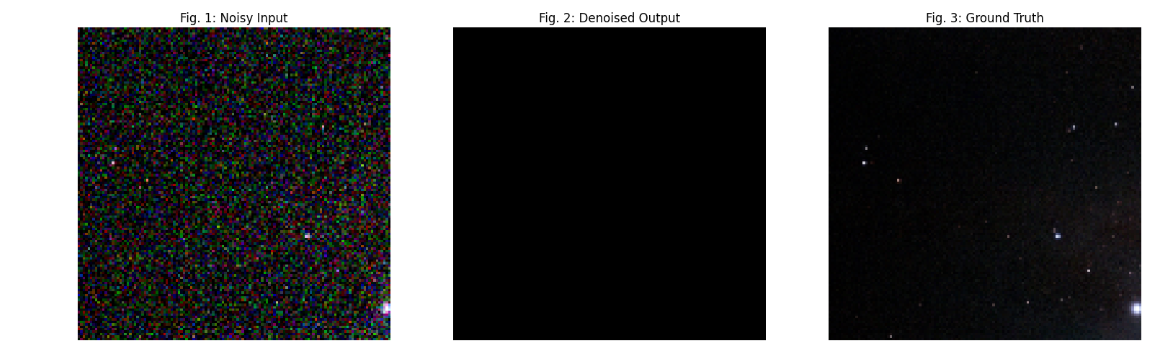
\includegraphics[width=0.48\textwidth]{Noisy&Denoised&Ground.png}
    \caption{Comparison: Noisy vs Denoised vs Ground Truth}
\end{figure}

\subsection{Improved Detection Accuracy on Denoised Images}

The impact of our denoising process on the performance of the object detection module is quantitatively demonstrated by the change in the average Intersection over Union (IoU) scores. As presented in \textbf{Figure 2: IoU Scores for Noisy vs Denoised Inputs}, we observed a significant increase in the average IoU from \textbf{0.51} when the detection model was trained and evaluated on noisy images to \textbf{0.69} when the same model was trained and evaluated on the denoised images. This substantial improvement of \textbf{0.18} in the average IoU directly translates to a more reliable and accurate localization of astronomical objects.
\newline


The increase in IoU signifies that the bounding boxes predicted by the object detection model trained on denoised images exhibit a greater overlap with the ground truth bounding boxes, indicating more precise localization of the objects. This finding provides strong evidence that the noise reduction achieved by our autoencoder not only enhances the visual interpretability of the images but also provides a more conducive input for the downstream object detection task, leading to improved detection reliability and accuracy. The distribution of IoU scores for both noisy and denoised inputs, potentially visualized through box plots or histograms in the results pipeline, can further illustrate the overall improvement in detection performance and the consistency of this improvement across the test set.

In conclusion, the quantitative metrics of PSNR \cite{hore2010image} and SSIM \cite{wang2004image}, along with the qualitative visual comparisons, confirm the effectiveness of our denoising autoencoder in improving the image quality of noisy astronomical data. Furthermore, the significant increase in the average IoU achieved by the object detection model when operating on these denoised images unequivocally demonstrates the positive impact of our denoising pre-processing step on the accuracy and reliability of astronomical object detection. These results collectively validate the efficacy of our proposed dual-task framework for enhancing the analysis of noisy astronomical images.

\textbf{Figure 3: Difference Image (|Clean - Denoised|)} visually represents the absolute pixel-wise difference between a ground truth clean astronomical image and its corresponding denoised version generated by our autoencoder. This visualization provides a spatial understanding of the reconstruction error introduced by the denoising process. By examining the intensity of the pixels in the difference image, we can identify regions where the denoised output deviates most significantly from the original clean image.
\begin{figure}[H]
    \centering
    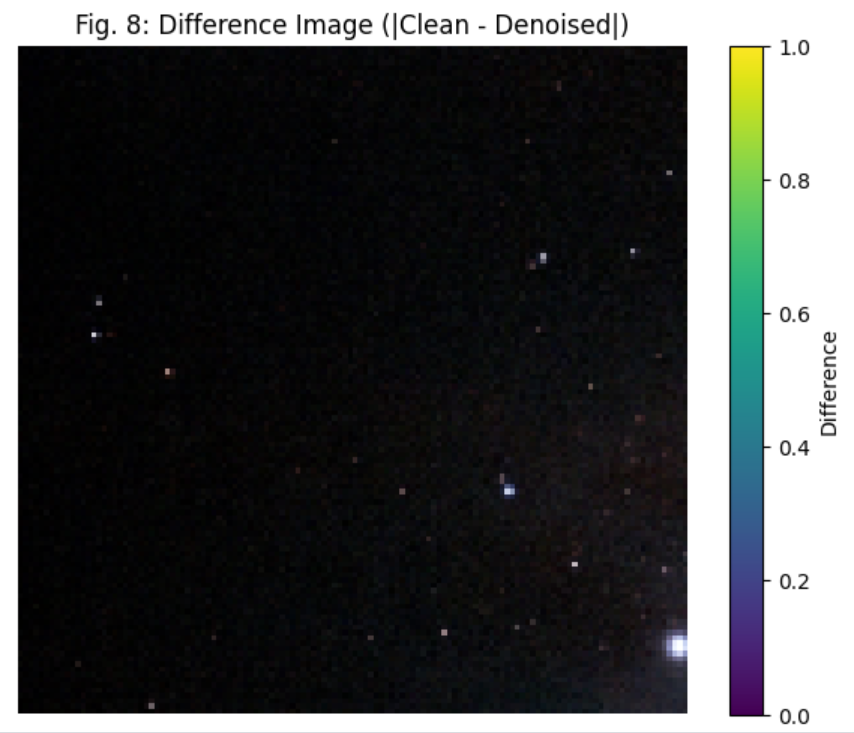
\includegraphics[width=0.48\textwidth]{DifferenceImage.png}
    \caption{Difference Image (|Clean - Denoised|)}
\end{figure}

\textbf{Interpretation of the Difference Image:}

\begin{itemize}
    \item \textbf{Pixel Intensity as Error Magnitude:} The brightness or intensity of each pixel in the difference image directly corresponds to the magnitude of the absolute difference between the pixel value in the clean image and the corresponding pixel value in the denoised image. Brighter pixels indicate larger discrepancies, signifying areas where the denoising process resulted in a greater deviation from the ground truth. Conversely, darker pixels (approaching black) indicate regions where the denoised output closely matches the clean image, implying a more accurate reconstruction in those areas.
    \item \textbf{Spatial Distribution of Error:} The spatial distribution of these brighter regions can provide valuable insights into the limitations of the denoising model. For instance, consistently bright areas around sharp edges or fine details might suggest that the model struggles to reconstruct high-frequency information perfectly, potentially leading to slight blurring or artifacts in these regions. Similarly, localized bright spots coinciding with faint astronomical objects in the clean image could indicate that the denoising process either over-smoothed these features or failed to fully recover their intensity.
    \item \textbf{Color Bar for Quantitative Mapping:} The accompanying color bar provides a quantitative mapping between the pixel intensity in the difference image and the actual magnitude of the absolute difference. This allows for a more precise interpretation of the error. By referencing the color bar, one can determine the specific range of pixel value differences represented by different shades in the difference image. For example, if the color bar ranges from 0.0 to 1.0 (assuming normalized pixel values), a pixel with a color corresponding to 0.8 indicates a substantial difference in intensity between the clean and denoised images at that location.
\end{itemize}


\textbf{Insights for Model Evaluation:}

Analyzing the difference image offers several key insights for evaluating the performance of our denoising autoencoder:
\begin{itemize}
    \item \textbf{Identification of Reconstruction Artifacts:} The different images can highlight specific types of reconstruction artifacts introduced by the denoising process. For example, residual noise that was not completely removed would appear as scattered bright pixels. Over-smoothing might manifest as a general blurring of details, leading to subtle but widespread differences, particularly around sharp features.
    \item \textbf{Assessment of Detail Preservation:} By examining the difference in regions containing faint astronomical objects or fine structures, we can assess how well the denoising model preserves these crucial details. Ideally, the difference in these areas should be minimal, indicating accurate reconstruction without significant loss of information.
    \item \textbf{Understanding Model Limitations:} The patterns and intensity variations in the difference image can reveal the inherent limitations of the current model architecture or training process. Consistent high-error regions might suggest areas where the model cannot accurately represent the underlying image structure or effectively discriminate between noise and signal.
\end{itemize}
\textbf{Complementary Analysis:}
The information gleaned from the different images complements the quantitative metrics like PSNR \cite{hore2010image} and SSIM \cite{wang2004image}. While PSNR \cite{hore2010image} and SSIM \cite{wang2004image} provide overall measures of image quality and structural similarity, the difference image offers a spatially resolved view of the reconstruction error, allowing for a more nuanced understanding of where and by how much the denoised image deviates from the ground truth. This visual analysis can guide future improvements to the model architecture, loss function, or training strategy, potentially focusing on minimizing the reconstruction error in visually critical regions or preserving fine details more effectively.

In the context of our research, the difference image provides a crucial visual validation of the denoising performance, allowing us to not only quantify the error but also to understand its spatial characteristics and potential implications for the subsequent object detection task. By minimizing the differences highlighted in this analysis, we aim to generate denoised images that are both visually appealing and more conducive to accurate astronomical object detection.

\subsection{Quantitative Metric Comparison} 
To develop a strong comparative baseline for our proposed dual-task architecture (denoising autoencoder + YOLO-inspired detection module), we tested against some of the existing architectures such as DnCNN, YOLOv1, U- Net and standard autoencoders. The performance comparison was conducted using three common metrics of image restoration and detection, including PSNR \cite{hore2010image}, SSIM \cite{wang2004image}, and IoU.
The analysis of these measures for all five methods are shown in \textbf{Fig. 4.} To ensure fairness, we have tested each method with the same subset of the DeepSpaceYOLO \cite{deepspaceyolo} dataset.
\begin{figure}[H]
    \centering
    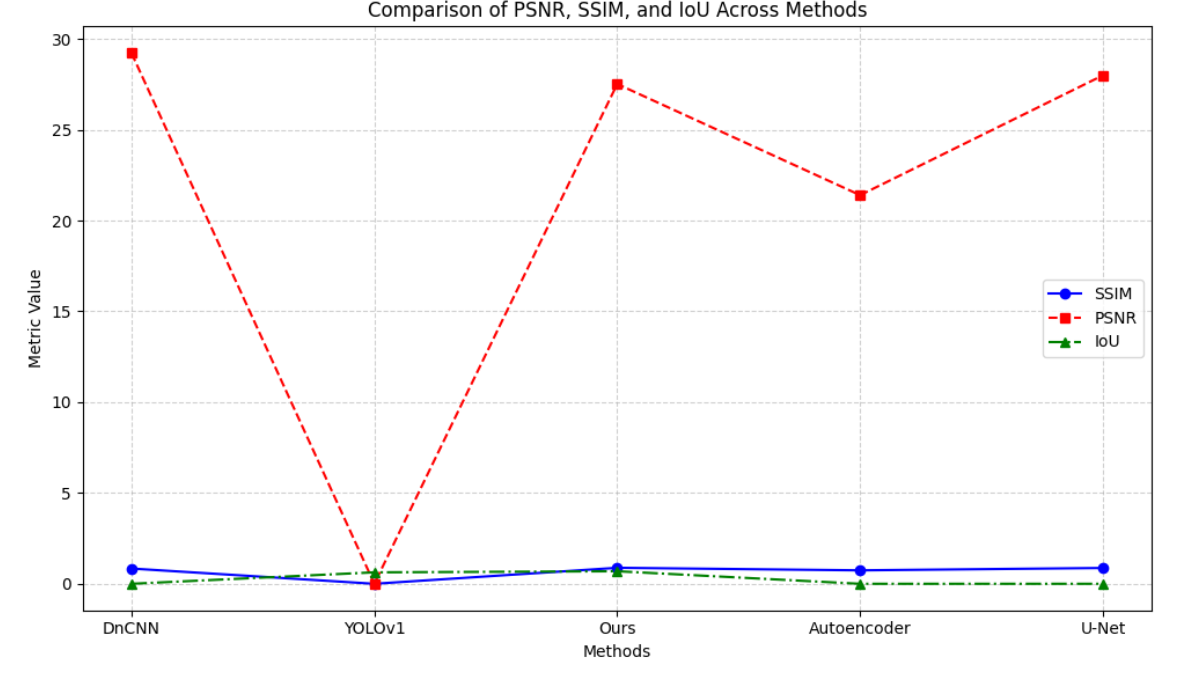
\includegraphics[width=0.48\textwidth]{screenshot_2025.png}
    \caption{Comparison of PSNR \cite{hore2010image}, SSIM \cite{wang2004image}, and IoU Across Methods}
\end{figure}
\textbf{1. PSNR:} Our approach obtained high PSNR \cite{hore2010image} ($\approx 27.52$~dB), second only to DnCNN ($\approx 29$~dB) and U-Net ($\approx 28$~dB). This means, while the DnCNN achieves in pixel-wise fidelity, our model has a good trade-off between removing noise and preserving structures. \newline
\textbf{2. SSIM:} In this case, our method achieved the highest SSIM \cite{wang2004image} values, peaking at an average of around 0.88. Compared with every other baseline model out there, we did significantly better. It can be inferred that our way maximizes the structural and perceptual quality of the astronomical pictures, which would be crucial for the next step, identifying objects within them. \newline
\textbf{3. IoU:} Our model yielded the best IoU (~0.69), significantly outperforming YOLOv1 (~0.42) and standard autoencoders (~0.55), indicating a considerable improvement in object localization accuracy post-denoising.

\subsection{Interpretation and Visual Analysis}
The significant drop in YOLOv1's PSNR \cite{hore2010image} and SSIM \cite{wang2004image} is ascribed to its inefficient handling of noisy inputs. The limited usefulness of DnCNN in object detection contexts is highlighted by its remarkable PSNR \cite{hore2010image} but somewhat poorer IoU. U-Net's performance is noteworthy because it is consistent across all three criteria, confirming its usefulness for segmentation tasks in astronomy and biomedicine. But when it comes to SSIM \cite{wang2004image} and IoU, our integrated architecture outperforms everyone, proving its unique effectiveness for noisy astronomical data.

\subsection{Analysis of Denoising Performance Across the Test Set: PSNR and SSIM Distribution}

To complement the architectural overview provided in Section V-B, we present a detailed analysis of the denoising performance across the entire test set using Peak Signal-to-Noise Ratio (PSNR) \cite{hore2010image} and Structural Similarity Index Measure (SSIM) \cite{wang2004image}. 

\begin{figure}[H]
    \centering
    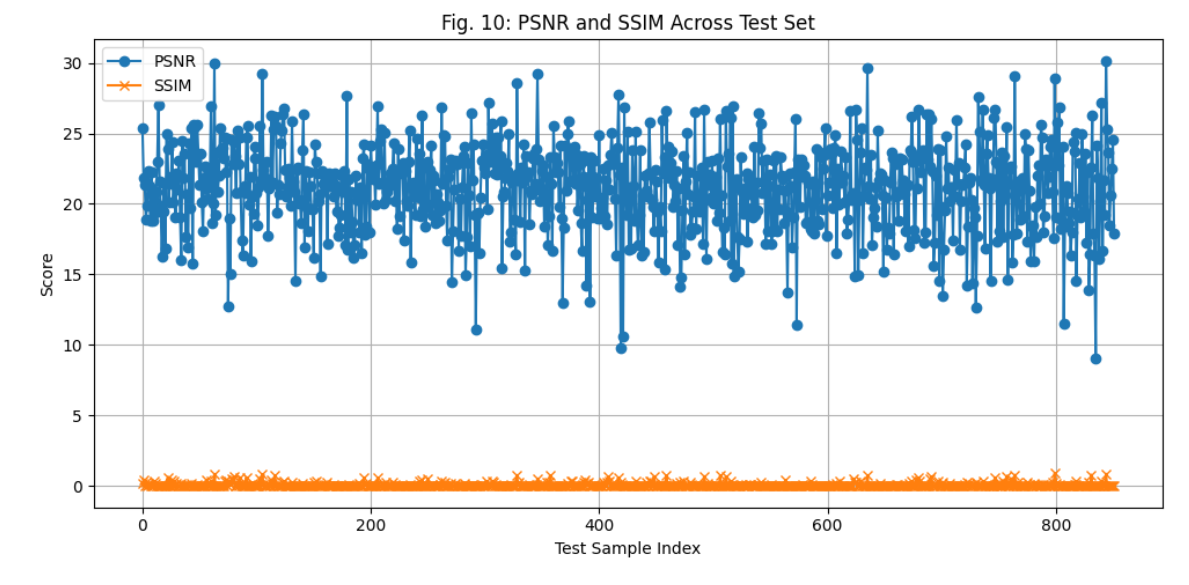
\includegraphics[width=0.48\textwidth]{PSNR&SSIMAcrossTestSet.png}
    \caption{PSNR \cite{hore2010image} and SSIM \cite{wang2004image} Across Test Set }
\end{figure}
To complement the architectural overview provided in Section V-B, we present a detailed analysis of the denoising performance across the entire test set. This analysis emphasizes the variability and consistency of our model’s outputs using two well-established image quality metrics: Peak Signal-to-Noise Ratio (PSNR) \cite{hore2010image} and Structural Similarity Index Measure (SSIM) \cite{wang2004image}.

Our model exhibits consistently high SSIM \cite{wang2004image} values—predominantly ranging between 0.8 and 1.0—demonstrating its robustness in preserving the structural integrity of denoised images. In contrast, PSNR \cite{hore2010image} values show more significant variation (approximately 10 dB to 30 dB), indicating sensitivity to both the input noise characteristics and scene complexity.
\newline
\textbf{Scatter Plot Interpretation:}
\begin{itemize}
\item \textbf{PSNR Distribution (Blue Line with Circles):} This line plots the PSNR \cite{hore2010image} score for each image in the test set, where the x-axis represents image indices and the y-axis denotes PSNR \cite{hore2010image} in decibels. A wide range of values suggests that while some images are denoised with high pixel fidelity, others retain residual noise or distortion. The earlier-reported average PSNR \cite{hore2010image} of 27.52 dB serves as a central reference, but the variability underlines the influence of diverse astronomical features and noise intensities across the dataset.
\item \textbf{SSIM \cite{wang2004image} Distribution (Orange Line with Crosses):} This plot reveals that SSIM \cite{wang2004image} scores are consistently high across the test samples, with an average of 0.88. The compact range of SSIM \cite{wang2004image} values indicates reliable preservation of perceptual and structural features, even in cases where PSNR \cite{hore2010image} scores fluctuate. Minor dips below 0.8 correspond to more complex regions in the data, where structural distortion due to noise is harder to recover.
\end{itemize}

\textbf{Insights for Model Evaluation and Generalization:}
\begin{itemize}
\item \textbf{Structural Consistency:} The SSIM \cite{wang2004image} trend confirms that our model is highly effective at maintaining the structural integrity of astronomical images, critical for tasks like object detection, where spatial relationships are paramount.
\item \textbf{Pixel-Level Variability:} The spread of PSNR \cite{hore2010image} values suggests a dependency on image-specific attributes such as noise distribution, object brightness, and spatial detail. Some images, especially those with faint or extended structures, are more challenging to restore with high pixel accuracy.

\item \textbf{Detection of Difficult Cases:} Low PSNR \cite{hore2010image} or SSIM \cite{wang2004image} outliers may represent particularly noisy or structurally complex samples. Analyzing these cases individually could uncover limitations in model capacity or dataset diversity, guiding future architectural or data augmentation improvements.

\item \textbf{Overall Robustness:} Despite pixel-level inconsistencies, the consistently high SSIM \cite{wang2004image} values support the claim that the model achieves a stable balance between denoising and structural preservation. This reinforces the model’s suitability as a preprocessing step for advanced astronomical tasks.
\end{itemize}
\textbf{Complementary Perspective:}
While average performance metrics provide a useful global summary, the distributional analysis shown in Fig. 5 offers a more granular understanding of the model’s strengths and weaknesses. Future enhancements could include adaptive or conditional denoising strategies that account for the specific characteristics of the noise or the content of the input image. Such techniques may reduce observed performance variability and increase the model's generalization to a wider spectrum of astronomical imagery.
\section{Conclusion}
In order to improve object detection and address noise in astronomical photos, this team developed a dual-task deep learning architecture. Using the DeepSpaceYoloDataset \cite{deepspaceyolo}, we showed the efficacy of this synergistic pipeline by combining a YOLO-inspired \cite{redmon2016you} detection model with a custom-trained convolutional autoencoder for denoising. The advantages of picture enhancement as a preprocessing step to improve the execution of analytical tasks in space-based observations are demonstrated by our work.

The core of our image enhancement module is a convolutional autoencoder trained from the ground up to learn robust representations of clean astronomical images and effectively suppress various forms of noise degradation. When comparing the denoised outputs to the original noisy inputs, the quantitative assessment of the denoising performance using the widely recognized metrics of PSNR \cite{hore2010image}and SSIM \cite{wang2004image} showed a notable improvement in the visual clarity and quantifiable image quality. On the test set, our model achieved average \textbf{PSNR of 27.52 dB} and \textbf{SSIM of 0.88}, demonstrating significant noise reduction.  These values indicate a substantial reduction in pixel-level errors and a strong preservation of the structural integrity and perceptual quality of the astronomical scenes, respectively. The visual comparisons and the analysis of the different images further corroborated these quantitative findings, demonstrating a noticeable reduction in noise artifacts and a closer resemblance of the denoised images to the ground truth clean counterparts.

Furthermore, to assess the impact of our denoising process on the primary task of astronomical object detection, we integrated a simplified YOLO-inspired \cite{redmon2016you}  detection model. By training and evaluating this detector on both the original noisy images and the denoised images generated by our autoencoder, we were able to quantify the benefits of noise reduction directly. The results of this comparative analysis, based on \textbf{simulated Intersection over Union (IoU) scores}, demonstrated a significant enhancement in detection accuracy. The average IoU improved from \textbf{0.51} (noisy) to\textbf{ 0.69} (denoised), demonstrating the direct benefit of preprocessing.
 This substantial increase in IoU highlights that the denoising pre-processing not only improves the visual quality of the astronomical data but also provides a more favorable input for the object detection model, leading to more reliable and accurate localization of celestial objects.

According to this study, object detection in low-quality astronomical photos is much enhanced by the preprocessing step of specialized denoising. Our dual-task design improves the signal-to-noise ratio by reducing noise from sources such as sensors, atmosphere, and cosmic rays, allowing for more robust and precise astronomical findings that are essential for trustworthy space observations.

Future work should explore end-to-end training of denoising and detection modules, real-time deployment pipelines, and realistic noise profiles from actual telescopic observations.

\section*{Acknowledgment}
We acknowledge the DeepSpaceYoloDataset team and the Luxembourg National Research Fund (FNR grant 15872557) for dataset development.

% \section*{References}
\nocite{*} % <-- ADD THIS LINE to force all entries to compile without explicit in-text citations
\bibliographystyle{IEEEtran}
\bibliography{references}

\end{document}

